\documentclass[landscape]{ximera}
%\documentclass[landscape]{article}
\input{../preamble.tex}
\input{../preambles/poster.tex}
%\input{../preambles/linalg}
\addPrintStyle{..}

\begin{document}
    \author{Zomercursus KU Leuven}
    \xmtitle{Complexe getallen}{}
    \label{steekkaart:complexe_getallen}

\tikzset{>=latex}	
\renewcommand{\important}[1]{\ensuremath{\fcolorbox{kuaccent!50!white}{kuaccent!50!white}{$#1$}}}   % HACK: NO border ...

\begin{tcbposter}
    
\xmpostertitle{Complexe getallen: definities en eigenschappen}{span=6}

\posterbox[adjusted title={Definitie en schrijfwijzen (met $a,b\in\R, r\in\Rplus, \theta\in\left[0,2\pi\right]$)}]{
	name=l1,column=1,span=6,below=title,
}{
	Definitie: $\important{\C} = \{a+bi\mid| a,b\in\R, i^2= -1\}$ is de verzameling van de \textbf{complexe  getallen}.
	\\
	\scalebox{0.9}{
	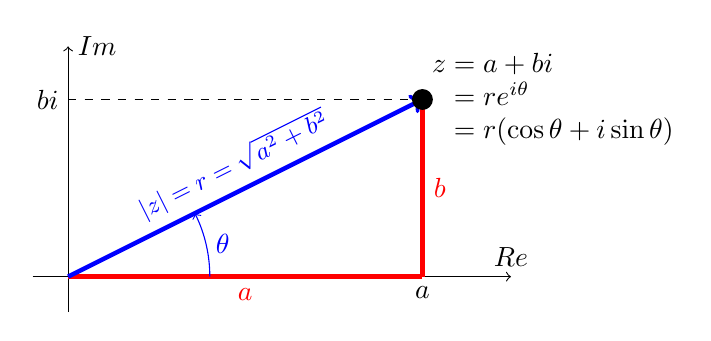
\begin{tikzpicture}[scale=2.25,baseline=(current bounding box.center)]
	
	\draw[thin,->] (-0.2,0)  -- (2.5,0) node[above] {$Re$};
	\draw[thin,->] (0,-0.2)  -- (0,1.3) node[right] {$Im$};
	
	\draw[gray,thin,dashed] (0,1) -- (2,1);
	\draw[gray,thin,dashed] (2,0) -- (2,1) ;
	
	\draw[dashed] (0,1) -- (2,1)node[right,align=left] {$z=\red{a}+\red{b}i$\\$\phantom{z}= \blue{r}e^{i\blue{\theta}}$\\$\phantom{z} = \blue{r}(\cos\blue{\theta}+i \sin\blue{\theta})$}; 
	
	\draw[color=red,ultra thick] (0,0)  --  node[below]{$a$} (2,0);
	\draw (2,0)node[below]{$a$};
	\draw[color=red,ultra thick] (2,0)  --  node[right]{$b$} (2,1);
	\draw (0,1) node[left]{$bi$};
	
	\draw[color=blue,ultra thick, ->] (0,0) -- node[above,sloped]{\small$|z|=r=\sqrt{a^2+b^2}$ } (2,1);
	\draw[color=blue, ->] (0.8,0) arc (0:atan(0.5):0.8) node [midway,right] {$\theta$}; 		

	\node at (2,1) [circle, fill=black, scale=0.8]{};    % last to put it ON TOP of arrows...
	\end{tikzpicture}
	}
	\begin{tabular}{l@{}ll}
		cartesisch: & \important{z=\red{a+bi}} \\
		(of algebraïsch) &\\
		polair: & \important{z=\blue{r(\cos\theta+i\sin\theta)}} & \\
		(of goniometrisch) &\\
		exponentieel: & \important{z=\blue{re^{i\theta}}} & 
	\end{tabular}

	\begin{tabular}{llllll}
	met & $a=Re(z)$ & het \textbf{reëel deel}, 
	& en  & $r=|z|$ & de \textbf{norm} of \textbf{modulus} 
	\\
	    & $b=Im{z}$ & het \textbf{imaginair deel},
	&   & $\theta$  & het \textbf{argument} of de \textbf{fase}.
	\end{tabular}

	\begin{tabular}{llll}
	Hierbij is & 
	\important{e^{i\theta} = \cos \theta + i \sin \theta} & (Formule van Euler) 
	 & (en dus $e^{-i\theta} = \cos \theta - i \sin \theta$) \\
	en dus & \important{\cos \theta=\dfrac{e^{i\theta}+e^{-i\theta}}{2}}
	       & en \important{\sin \theta=\dfrac{e^{i\theta}-e^{-i\theta}}{2i}} \\[5mm]
\end{tabular}


}



\posterbox[adjusted title=Omzettingsformules]{
    name=l2,column=1,span=6,below=l1,
}{

\begin{tabular}{rlrl}
	Van $r,\theta$ naar $x,y$: & \important{x =  r \cos \theta} & 
	Van $x,y$ naar $r,\theta$: &  \important{r = \sqrt{x^2+y^2}} \\
	& \important{y =  r \sin \theta} & 
	& \important{\tan\theta  = \dfrac{y}{x}}  \quad (als $x\neq0$)
%	  en dus & \important{\cos\theta  = \dfrac{x}{\sqrt{x^2+y^2}}} en \important{\sin\theta  = \dfrac{y}{\sqrt{x^2+y^2}}} \\
\end{tabular}

% \begin{tabular}{rll}
% 	Van $r,\theta$ naar $x,y$: & \important{x =  r \cos \theta}\\
% 							   & \important{y =  r \sin \theta} \\[3mm]
% 	Van $x,y$ naar $r,\theta$: &  \important{r = \sqrt{x^2+y^2}} 
% %	  en dus & \important{\cos\theta  = \dfrac{x}{\sqrt{x^2+y^2}}} en \important{\sin\theta  = \dfrac{y}{\sqrt{x^2+y^2}}} \\
% 	  & en dus $\cos\theta  = \frac{x}{\sqrt{x^2+y^2}}$ en $\sin\theta  = \frac{y}{\sqrt{x^2+y^2}}$, of \\[-3mm]
% 	  & \important{\tan\theta  = \dfrac{y}{x}}  & (als $x\neq0$)
% \end{tabular}

Een rekenmachine geeft voor $\bgtan\tfrac{y}{x}$ een hoek tussen $-\tfrac{\pi}{2}$ en $\tfrac{\pi}{2}$, dus waarvoor $x>0$. 
\\ \textbf{Als $x<0$ moet je dus $\pi$ bijtellen. Maak altijd een tekening/schets !}
\\ Er geldt ook  $\cos\theta  = \frac{x}{\sqrt{x^2+y^2}}$ en $\sin\theta  = \frac{y}{\sqrt{x^2+y^2}}$.

% \textbf{polair/exponentieel $\rightarrow$ cartesiaans}: $a=r\cos\theta$, $b=r\sin\theta$

% \textbf{cartesiaans $\rightarrow$ polair/exponentieel}: $r=|a+bi|=\sqrt{a^2+b^2}$

% \begin{minipage}[t]{12cm}
% $$	\begin{array} {lll}
% 		\text{Voor }a>0:& \theta = \mbox{Atan}\left(\frac{b}{a}\right)\hspace{7cm}\mbox{}\\
% 		\text{Voor }a<0:
% 		&\theta = \mbox{Atan}\left(\frac{b}{a}\right)+\pi\\
% 		\text{Voor }a=0:                  
% 		&\theta  = \frac{\pi}{2}\text{, als }b>0 \\
% 		&\theta  = -\frac{\pi}{2}\text{, als }b<0
% 	\end{array}
% $$
	% \textbf{Slagzin}: Teken het punt in het complexe vlak. \\
	% Op de imaginaire as geen boogtangens nodig. \\
	% Let op $\bgtan(b/a)$ versus $\bgtan(b/a)+\pi$ rechts en links van de imaginaire as.

	% %\end{minipage}
	
}

\posterbox[adjusted title=Voorbeelden]{
	name=l3,column=1,span=6,below=l2
}{


\textbf{Soms loont het $z$ om te zetten naar een vorm waarin een bewerking eenvoudiger is.}


	\scalebox{0.85}{
	\begin{tikzpicture}[scale=2,baseline=(current bounding box.center)]
	
	\tikzmath{\hoek = 20; \myc = cos(\hoek); \mys = sin(\hoek); 
		\hoekb = 20;}
	
	
	% Goniometrische cirkel
	\draw (0,0) circle (1cm);
	\draw[gray,->] (-1.2,0) -- (1.2,0);% node[right] {$x$};
	\draw[gray,->] (0,-1.2) -- (0,1.2);% node[above] {$y$};
	%	\draw  (0, 0) node [below left]  {$(0,0)$};
	\draw  ( 1,  0) node [align=right,below right] {$\blue{e^{i0}} = e^0 $\\$= 1$\\$=\red{1+0i}$};
	\draw  (-1,  0) node [align=left,below left]  {$\blue{e^{i\pi}} = e^{-i\pi} $\\$= -1$\\$=\red{-1+0i}$};
	\draw  ( 0,  1) node [align=right,above ]  {$\blue{e^{i\pi/2}} = i=\red{0+1i}$};
	\draw  ( 0, -1) node [align=right,below ]  {$\blue{e^{-i\pi/2}} = -i=\red{0-1i}$};
	\draw[blue]  (0,0) -- (45:1) node [align=left, right]  {\ $\blue{e^{i\pi/4}} =$\\\ $\red{\tfrac{\sqrt{2}}{2} + i \tfrac{\sqrt{2}}{2}}$};
	\draw[blue]  (0,0) -- (150:1) node [align=right,left]  {$\blue{e^{i5\pi/6}} =\ $\  \\$\red{-\tfrac{\sqrt{3}}{2} + \tfrac{1}{2}i}\ $\ };
	\draw[thin, dashed, blue]  (0,0) -- (-30:1);
	% \draw[blue,dashed]  (0,0) -- (45:1) node [above right]  {$\color{blue}\alpha=\frac{\pi}{4}$};
	% \draw[blue,dashed]  (0,0) -- (-45:1) node [below right,align=left]  {$\color{blue}\alpha=-\frac{\pi}{4}$\\$\alpha=\frac{7\pi}{4}$};
	% \draw[blue,dashed]  (0,0) -- (60:1) node [above]  {$\color{blue}\alpha=\frac{\pi}{3}$};
	% \draw[blue,dashed]  (0,0) -- (135:1) node [above left]  {$\color{blue}\alpha=\frac{3\pi}{4}$};		
	%
	\node at (0,1) [circle, fill=black, scale=0.6]{};  
	\node at (1,0) [circle, fill=black, scale=0.6]{};  
	\node at (-1,0) [circle, fill=black, scale=0.6]{};  
	\node at (0,-1) [circle, fill=black, scale=0.6]{};  
	\node at (45:1) [circle, fill=black, scale=0.6]{};  
	\node at (150:1) [circle, fill=black, scale=0.6]{};  
	\end{tikzpicture}
	}
	%\hfill
\begin{tabular}{@{ }r@{ }r@{ }l@{ }l@{ }}
	 $1=$ & $1+0i$ & $= e^{i0} = e^{i 2\pi}$, \\
	 $i=$ & $0+1i$ & $= e^{i\frac{\pi}{2}} = \left(e^{i\pi}\right)^{1/2} = \sqrt{e^{i\pi}} = \sqrt{-1}$, \\
	 $-1=$ & $-1+0i$ & $= e^{i\pi} = e^{-i\pi}$, \\
	 $-i=$ & $ 0-1i$ & $= e^{-i\frac{\pi}{2}}=e^{i\frac{3\pi}{2}}=\left(e^{i\pi/2}\right)^{-1}=i^{-1} = \frac{1}{i}$\\
	 \multicolumn{2}{r}{$\tfrac{\sqrt{2}}{2} + \tfrac{\sqrt{2}}{2}i$} & $= e^{i\frac{\pi}{4}}=\cos\frac{\pi}{4} + i\sin\frac{\pi}{4}$ \\
	 \multicolumn{2}{r}{$-\tfrac{\sqrt{3}}{2} + \tfrac{1}{2}i$} & $=e^{i\frac{5\pi}{6}}=\cos\frac{5\pi}{6} + i\sin\frac{5\pi}{6}$ \\
	 \multicolumn{4}{r}{\textbf{\red{PAS OP:}} $\arctan(-\tfrac{\sqrt{3}}{3})$ op je rekenmachine geeft } \\
	 \multicolumn{4}{r}{de hoek $-\tfrac{\pi}{6} = -0.5235\ldots$. Je moet $\pi$ bijtellen!} \\
\end{tabular}

		%\textbf{algebra\"ische of cartesiaanse vorm}, a,b\in\R, i^2=-1.
% 	\important{\makebox[4.5cm][l]{$Re(a+bi)=a$}} & \qquad &
% 	\textbf{re\"eel deel}
% 	\\
% 	\important{\makebox[4.5cm][l]{$Im(a+bi)=b$}} & \qquad &
% 	\textbf{imaginair deel} 
% 	\\
% 	\important{\makebox[4.5cm][l]{$r=|z|=|a+bi|=\sqrt{a^2+b^2}$}} & \qquad &
% 	\textbf{modulus of norm} \\
% 	\important{\makebox[4.5cm][l]{$\theta$}} & \qquad &
% 	\textbf{argument of fase} \\
% \end{array}
% $
}

\posterbox[adjusted title=Complex toegevoegde en modulus]{
	name=r1,column=7,span=6,below=title
}{

\begin{tabular}{ll}
\textbf{Norm} of \textbf{modulus}: & \important{|z|=|a+bi|=\sqrt{a^2+b^2} = |re^{i\theta}| = r} \\
\textbf{Complex toegevoegde}:      & \important{\overline z=a-bi = r(\cos\theta -i \sin\theta) = r(\cos (-\theta)+i \sin (-\theta))  = re^{-i \theta}} \\
\end{tabular}

% \textbf{Complex toevoegen}

\scalebox{0.8}{
\begin{tikzpicture}[scale=1.5,baseline=(current bounding box.center)]%,cap=round,transform canvas={scale=0.5}]
	
	\draw[thin,->] (-0.3,0)  -- (2.5,0) node[above] {$Re$};
	\draw[thin,->] (0,-1.1)  -- (0,1.3) node[right] {$Im$};
	
	
	\draw[dashed] (0,1) -- (2,1)node[above] {$z=a+bi=re^{i \theta}$}; 
	\draw[dashed] (2,-1) -- (2,1) ;
	\draw[dashed] (0,-1) -- (2,-1); 
	
	
	\draw[blue,ultra thick, ->] (0,0) -- node[red,above, sloped]{\important{|z|=r}} (2,1);
	\draw[->] (0.8,0) arc (0:atan(0.5):0.8) node [midway,right] {$\theta$}; 	
	
	\draw[color=red,ultra thick, ->] (0,0) -- node[teal,below]{$r$} (2,-1);
	\draw[color=teal, ->] (0.8,0) arc (0:atan(-0.5):0.8) node [midway,right] {$-\theta$}; 		
	
	\draw (2,0)node[below]{$a$};
	\draw (0,1) node[left]{$bi$};
	\draw (0,-1) node[left]{$-bi$};

	\node at (2,1) [circle, fill=black, scale=0.3]{};
	\node at (2,-1) [circle, fill=black, scale=0.3]{};
	\draw[red]	(2,-1) node[above right] {\important{\overline z=a-bi = re^{-i \theta}}};
	% \draw (2,-1.4) node[right] {\textbf{complex toegevoegde}};
	
	\draw (4.2,1) node[below right]{\large
	$
	\begin{array}{ll}
			z+\bar z &= 2a\\
			z-\bar z &= 2b\\
			z \bar z &=a^2+b^2\\
					  &=r^2\\
			z / \bar z &= e^{2i\theta}
	\end{array}
	%$
	%\textbf{eigenschappen modulus}
	\qquad
	%$ 
	\begin{array}{ll}
		|z_1 z_2| &= |z_1| |z_2|\\
		\left|\frac{z_1}{z_2}\right| &= \frac{|z_1|}{|z_2|}\\ \\
		|z^n| &= |z|^n
	\end{array}
	$	
	};

\end{tikzpicture}
}


\begin{tabular}{llllll}
	\textbf{Slagzin}: & overal \(i\) vervangen door \(-i\) & \quad & % \\
	\textbf{Grafisch}:& spiegelen omheen de re\"ele as. \\
\end{tabular}

% \textbf{Soms loont het $z$ om te zetten naar een vorm waarin een bewerking eenvoudiger is.}

}

\posterbox[adjusted title=Tweedegraadsvergelijking met re\"ele co\"effici\"enten]{
	name=r2,column=7,span=6,below=r1
}{	

Vergelijking $ax^2+bx+c=0$ met $\blue{a,b,c \in \R}$ en $D = b^2-4ac$ heeft twee oplossingen $x_1$ en $x_2:
$

\begin{tabular}{lll}
als $D> 0$: 
		& $x_1 = \frac{-b + \sqrt{D}}{2a}$ en $x_2 = \frac{-b - \sqrt{D}}{2a}$
		& \textbf{verschillend en re\"eel}\\[2mm]
als $D= 0$: 
		& $x_1 = x_2 =\frac{-b}{2a}$ 
		& \textbf{samenvallend en re\"eel} \\[2mm] % (tweevoudig nulpunt)\\
als $D< 0$: 
		& $x_1 = \frac{-b + i\sqrt{|D|}}{2a}$ en $x_2 = \frac{-b - i\sqrt{|D|}}{2a}$
		& \textbf{complex toegevoegd}\\	
\end{tabular}
}

\posterbox[adjusted title=Tweedegraadsvergelijking met complexe co\"effici\"enten]{
	name=r3,column=7,span=6,below=r2
}{	
	
	Vergelijking $ax^2+bx+c=0$ met $\blue{a,b,c \in \C}$ en $D = b^2-4ac$ heeft twee oplossingen $x_1$ en $x_2$
	
	met altijd $x_1 = \frac{-b +  \sqrt{D}}{2a}$ en $x_2 = \frac{-b - \sqrt{D}}{2a}$,
    met $\sqrt{D}$ een (complexe) wortel van $D$.
}


\posterbox[adjusted title=Hoofdstelling van de algebra]{
	name=r4,column=7,span=6,below=r3
}{	

\textbf{Elke veelterm heeft over $\C$ een ontbinding in lineaire factoren.} \\
Gevolg (of equivalent): een veelterm van graad $n$ heeft precies $n$ nulpunten (met multipliciteiten).

Voor elke veelterm \(a_n x^n + a_{n-1} x^{n-1} + \ldots + a_1 x + a_0\) van graad \(n\) (dus \(a_n\neq 0\)),\\
	met coëfficiënten \(a_i\in\mathbb{C}\), bestaan er 
		getallen \(z_1,z_2,\ldots,z_n \in\mathbb{C}\), zodat
$$
	\important{a_n x^n + a_{n-1} x^{n-1} + \ldots + a_1 x + a_0=a_n(x-z_1)(x-z_2)\ldots(x-z_n)}.
$$
De getallen \(z_1,z_2,\ldots,z_n\) zijn dus nulpunten (of wortels) van de 
		veelterm,\\
	d.w.z. oplossingen van de vergelijking 
$
	a_n x^n + a_{n-1} x^{n-1} + \ldots + a_1 x + a_0=0.
$
}

\end{tcbposter}


\begin{tcbposter}
	\xmpostertitle{Complexe getallen: bewerkingen}{span=4}
	
	
	\posterbox[adjusted title=Optellen / som]{
		name=l1,column=1,span=4,below=title
	}{
	
	%\textbf{Optellen / Som} 
	
	\begin{tikzpicture}[scale=1.5]
		
		\draw[thin,->] (-0.2,0)  -- (3.5,0) node[above] {$Re$};
		\draw[thin,->] (0,-0.2)  -- (0,2.3) node[right] {$Im$};
		
		\draw[blue,ultra thick, ->] (0,0) --  (3,2  ) coordinate (z1) node[above left]{$z_1=a+bi$};	
		\draw[blue,ultra thick, ->] (0,0) --  (2,0.5) coordinate (z2) node[below right]{$z_2=c+di$};	
		
		% \draw[color=red,ultra thick, ->] (0,0) -- (3,2);
		\draw[color=red,ultra thick, ->] (0,0) -- ($(z1)+(z2)$) node[above]{$z_1+z_2$};
		\draw[color=red] (0,3) node[right]{\important{z_1+z_2=(a+c)+(b+d)i}};
		\draw[dashed] (z2) -- ($(z1)+(z2)$) ;
		\draw[dashed,ultra thick, color=blue,->] (z1) -- ($(z1)+(z2)$);	
		%\draw (3,1.6) node[right] {\textbf{som}};	
		
	\end{tikzpicture}
	
	\begin{tabular}{ll}
	\textbf{Slagzin}: & Som van de reële delen, \\
	                  & som van de imaginaire delen.\\
	\textbf{Grafisch}:& Pijlen na elkaar zetten. \\
	\textbf{Polair}:  & Omzetten naar cartesiaans.
	%% \textbf{Polair}:& $re^{i\alpha}+se^{i\beta} = ???$ (geen eenvoudige formule).

	\end{tabular}
	
	}
	\posterbox[adjusted title=Aftrekken / verschil]{
		name=l2,column=1,span=4,below=l1    % could be r1, but must be replaced !
	}{
		
	%\textbf{Aftrekken}
	
	
	\begin{tikzpicture}[scale=1.5]
		
		\draw[thin,->] (-0.2,0)  -- (3.5,0) node[above] {$Re$};
		\draw[thin,->] (0,-0.2)  -- (0,2.3) node[right] {$Im$};
		
		\draw[blue,ultra thick, ->] (0,0) -- (3,2  ) coordinate (z1) node[right]{$z_1=a+bi$};
		\draw[blue,ultra thick, ->] (0,0) -- (2,0.5) coordinate (z2) node[below right]{$z_2=c+di$};

%		\draw[dashed] (1,1.5) -- (3,2) ;
		\draw[color=red,ultra thick, ->] (0,0) -- ($(z1)-(z2)$) node[above] {$z_1-z_2$};
		\draw[dashed, color=blue,ultra thick, ->] (z1) -- node[above left] {$-z_2$} ($(z1)-(z2)$);
		\draw[color=red] (0,3) node[right]{\important{z_1-z_2=(a-c)+(b-d)i}};
		%\draw[color=red,ultra thick, ->] (2,0.5) -- ($(z1)-(z2)$);	
		%\draw[color=teal,ultra thick, ->] (0,0) -- (1,1.5);	
		%\draw (2.7,1) node[right] {\textbf{verschil}};	
		
		% \draw[color=blue,<-] (1,1.5) -- (3,2) ;
%		
		\draw[color=teal,thin,dashed,->] (z2)  -- ($(z2)+(1.5,0)$) node[above] {$Re$};
		\draw[color=teal,thin,dashed,->] (z2)  -- ($(z2)+(0,1.9)$) node[right] {$Im$};
		\draw[color=red,thick,dashed,->] (z2)  -- (z1) node[right] {};
		
		
	\end{tikzpicture}
	
	\begin{tabular}{ll}
		\textbf{Slagzin}: & Verschil van de reële delen, \\
						  & verschil van de imaginaire delen.\\
		\textbf{Grafisch}:& Eindpunten met mekaar verbinden. \\
		\textbf{Polair}:  & Omzetten naar cartesiaans.
	\end{tabular}
	
}
	
\posterbox[adjusted title=Vermenigvuldigen / product]{
	name=r1,column=5,span=4,below=title
}{	
	
	
%	\begin{minipage}[t]{12cm}
%		$(a+bi)(c+di)=(ac-bd)+(ad+bc)i$\\
%		$ r(\cos\alpha+i\sin\alpha) \cdot s(\cos  \beta+i\sin\beta)=rs(\cos(\alpha+\beta)+i\sin(\alpha+\beta))
%		$\\
%		$
%		re^{i\alpha}se^{i\beta}=rse^{i(\alpha+\beta)}
%		$
%	\end{minipage}

	
		
	\begin{tikzpicture}[scale=1.5]%,cap=round,transform canvas={scale=0.5}]
		
		\draw[thin,->] (-0.2,0)  -- (2.5,0) node[above] {$Re$};
		\draw[thin,->] (0,-0.2)  -- (0,2.2) node[right] {$Im$};
		
		
		\draw[blue,ultra thick, ->] (0,0) -- (1,0.3)node[right] {$z_1=re^{i \alpha}$}; 
		\draw[blue,ultra thick, ->] (0,0) -- (2,1.5)node[right] {$z_2=se^{i \beta}$}; 
		\draw[color=red, ultra thick, ->] (0,0) -- node[left] {$rs$} (1.7,2.1) node[right] {$z_1z_2$};
		\draw[color=red] (5,2.3) node[left] {\important{z_1z_2=rse^{i (\alpha+\beta)}}}; 	
		% \draw (1.7,1.7) node[right] {\textbf{produkt}};
		
		\draw[->] (0.6,0) arc (0:atan(0.3):0.6) node [midway,right] {$\alpha$}; 
		\draw[color=teal,->] (0.766,0.230) arc (atan(0.3):atan(2.1/1.7):0.76) node [midway,right] {$\beta$}; 		
	\end{tikzpicture}
	
	\begin{tabular}{ll}
		\textbf{Slagzin}: & Product van de moduli, \\
						  & som van de argumenten.\\
		\textbf{Grafisch}:& modulus=schaalfactor, \\ 
		                  & argument=rotatiehoek (fasedraaiing) \\
		\textbf{Cartesiaans}: & \important{(a+bi)(c+di)=(ac-bd)+(ad+bc)i}  \\
		                      & dus: uitwerken met $i^2=-1$
	\end{tabular}

	
	
%	\hspace{1cm}\textbf{polair/exponentieel}
	
}

\posterbox[adjusted title=Delen / quotiënt]{
	name=r2,column=5,span=4,below=r1
}{	

%	\begin{minipage}[t]{12cm}
%		$\displaystyle{
%			\frac{a+bi}{c+di}=\frac{(a+bi)(c-di)}{(c+di)(c-di)}=\frac{ac+bd}{c^2+d^2}+\frac{bc-ad}{c^2+d^2}i
%		}$\\
%		$\displaystyle{
%			\frac{r(\cos(\alpha)+\sin(\alpha)i)}{s(\cos(\beta)+\sin(\beta)i)}=\frac{r}{s}(\cos(\alpha-\beta)+\sin(\alpha-\beta)i)
%		}$\\
%		$\displaystyle{
%			\frac{r e^{i\alpha}}{s e^{i\beta}} = \frac{r}{s} e^{i(\alpha - \beta)}
%		}$
%	\end{minipage}


	\begin{tikzpicture}[scale=1.5]%,cap=round,transform canvas={scale=0.5}]
	
	\draw[color=red,ultra thick, ->] (0,0) -- (1,0.3) node[right] {$\dfrac{z}{z_2}$};
	\draw[red]  (5,2.3) node[left] {\important{\frac{z_1}{z_2}=\frac{r}{s}e^{i (\alpha-\beta)}}}; 
	\draw[blue,ultra thick, ->] (0,0) -- (2,1.5) node[right] {$z_2=se^{i \beta}$}; 
	\draw[blue,ultra thick, ->] (0,0) -- (1.7,2.1) node[right] {$z_1=re^{i \alpha}$};

%	\draw (1.7,1.7) node[right] ;
%	
	\draw[->] (0.4,0) arc (0:atan(2.1/1.7):0.4) node [midway,right] {$\alpha$}; 
	\draw[color=teal,<-] (0.766,0.230) arc (atan(0.3):atan(2.1/1.7):0.76) node [midway,right] {$-\beta$}; 	

	\draw[thin,->] (-0.2,0)  -- (2.5,0) node[below] {$Re$};
	\draw[thin,->] (0,-0.2)  -- (0,2.5) node[right] {$Im$};	
	\end{tikzpicture}

	\begin{tabular}{@{}l@{}l@{}}
		\textbf{Slagzin}: & Quotiënt van de moduli, \\
						  & verschil van de argumenten.\\
		\textbf{Grafisch}:& modulus=schaalfactor, \\ 
		                  & argument=rotatiehoek (fasedraaiing) \\
		\textbf{Cartesiaans}: & \important{\frac{a+bi}{c+di}=\dfrac{(a+bi)\blue{(c-di)}}{(c+di)\blue{(c-di)}}=\dfrac{ac+bd}{c^2+d^2}+\frac{bc-ad}{c^2+d^2}i} \\
		                      & dus: teller en noemer maal \\
							  & complex toegevoegde van noemer.
	\end{tabular}

% \hspace{1cm}\textbf{polair/exponentieel}
}


\posterbox[adjusted title=Machten]{
		name=x1,column=9,span=4,below=title
}{	
	

%	\begin{minipage}[t]{12cm}
%	$r(\cos(\theta)+\sin(\theta)i)^n=r^n(\cos(n\theta)+\sin(n\theta)i)$
%	
%	$(re^{i\theta})^n=r^n e^{in\theta}$
%	\end{minipage}
	
	\begin{tikzpicture}[scale=1.5]%,cap=round,transform canvas={scale=0.5}]
	

	\draw [blue, ->, ultra thick,rotate=10] (0,0) --(1.3,0) node [right] {$z=re^{i\theta}$};
	
	\foreach \i in {2,3,...,6} 
		\draw [->, ultra thick,color=red,rotate=\i*10] (0,0) -- node [color=teal, above, rotate=\i*10,pos=0.9] {\small $r^{\i}$} (1.3^\i,0) node [right, black] {$z^{\i} = r^{\i}e^{i\i\theta}$};

		% \draw [->, ultra thick,color=teal,rotate=20] (0,0) --(1.69,0) node [right] {$z^2$};
		% \draw [->, ultra thick,color=teal,rotate=30] (0,0) --(2.197,0) node [right] {$z^3$};
		% \draw [->, ultra thick,color=teal,rotate=40] (0,0) --(2.856,0) node [right] {$z^4$};
		% \draw [->, ultra thick,color=teal,rotate=50] (0,0) --(3.713,0) node [right] {$z^5$};
		% \draw [->, ultra thick,color=teal,rotate=60] (0,0) --(4.827,0) node [right] {$z^6$};
	\draw[thin,->] (-0.2,0)  -- (2.5,0) node[below] {$Re$};
	\draw[thin,->] (0,-0.2)  -- (0,3) node[right] {$Im$};	
	
	\draw[red] (0,4.5) node[right] {\important{z^n=(re^{i\theta})^n=r^n e^{in\theta}}};
\end{tikzpicture}


\begin{tabular}{ll}
	\textbf{Slagzin}: & Modulus tot de \(n\)-de macht, \\ 
					  & argument maal \(n\) \\
	\textbf{Grafisch}:& modulus=schaalfactor, \\ 
					  & argument=rotatiehoek (fasedraaiing) \\
	\textbf{Cartesiaans}:& uitwerken (Binomium van Newton) \\ 
	                     & of omzetten naar polair \\ 
\end{tabular}
}

\posterbox[adjusted title=Wortels]{
		name=x2,column=9,span=4,below=x1
}{	

		$z=re^{i\theta}$ heeft precies $n$ n-demachtswortels:\\
		 $x_k = \sqrt[n]{r}e^{i\frac{\theta + k 2 \pi}{n}}$,  met $k=0,1,\ldots,n-1$

% \url{https://www.geogebra.org/m/By0RL6MI}

\centering

\scalebox{1}{
	\begin{tikzpicture}[scale=1.5,baseline=(current bounding box.center)]
	
	\tikzmath{\hoek = 20; \myc = cos(\hoek); \mys = sin(\hoek); 
		\hoekb = 20;}
	
	
	% Goniometrische cirkel
	\draw (0,0) circle (1cm);
	\draw[gray,->] (-1.2,0) -- (1.2,0);% node[right] {$x$};
	\draw[gray,->] (0,-1.2) -- (0,1.2);% node[above] {$y$};
	%	\draw  (0, 0) node [below left]  {$(0,0)$};
	\draw  (0,0) -- ( 0:1 ) node [align=right,above right] {$\blue{e^{0}} = 1$};
	\draw  (0,0) -- ( 72:1 ) node [align=right,above right] {$\blue{e^{i2\pi/5}}$};
	\draw  (0,0) -- ( 144:1 ) node [align=right,above left] {$\blue{e^{i4\pi/5}}$};
	\draw  (0,0) -- ( -144:1 ) node [align=right,below left] {$\blue{e^{i6\pi/5}}$};
	\draw  (0,0) -- ( -72:1 ) node [align=right,below right] {$\blue{e^{i8\pi/5}}$};
	\node at (0:1) [circle, fill=black, scale=0.6]{};  
	\node at (72:1) [circle, fill=black, scale=0.6]{};  
	\node at (144:1) [circle, fill=black, scale=0.6]{};  
	\node at (-144:1) [circle, fill=black, scale=0.6]{};  
	\node at (-72:1) [circle, fill=black, scale=0.6]{};  
	\end{tikzpicture}
}

Er zijn vijf 5-de wortels van $1$, namelijk $\important{e^{i2k\pi/5}}, k=0,1,2,3,4$.
}

\end{tcbposter}

\end{document}
